\documentclass[UTF8]{beamer}

\usepackage{ctex}

\usetheme{Madrid}
\usefonttheme[onlymath]{serif}
%\usecolortheme{}

\usepackage{tikz}
\usepackage{graphicx}
\usepackage{subfigure}
\usepackage{amsmath}
\usepackage{braket}

\usepackage{algorithm,algorithmic}

%information
\title{Husimi图}
\author{邴泓霖}

\begin{document}
\frame{\titlepage}
\begin{frame}\frametitle{目录}
    \tableofcontents
\end{frame}
%----------------------------------------------------------%
%
\section{论文中基本概念的梳理}
\subsection{流算符}
\begin{frame}\frametitle{流算符}
    在量子力学的课本中,在某一点的概率流算符(the probability flux)算符可以定义为
    \begin{equation}
        \hat{\mathbf{j}}_{\mathbf{r}} = \frac{1}{2m}(\ket{\mathbf{r}}\bra{\mathbf{r}}\hat{\mathbf{p}}+\hat{\mathbf{p}}\ket{\mathbf{r}}\bra{\mathbf{r}})           
        \label{flux:def}
    \end{equation}
    其中$\mathbf{r}$和$\mathbf{p}$分别是质量为$m$的粒子的位置和动量。
    
    同时,可以计算出概率流算符的平均值
    \begin{equation}
        \begin{aligned}
            \bra{\psi}\hat{\mathbf{j}}_{\mathbf{r}}\ket{\psi}&=
            \frac{\mathrm{i}\hbar}{2m}(
            \mathrm{\psi}(\mathbf{r})\nabla\mathrm{\psi}^{*}(\mathbf{r})
            -\mathrm{\psi}^{*}(\mathbf{r})\nabla\mathrm{\psi}(\mathbf{r})
            )\\
            &=\frac{1}{m}\Im[\mathrm{\psi}^{*}(\mathbf{r})(-\mathrm{i}\hbar\nabla)\mathrm{\psi}(\mathbf{r})]\\ 
            &=\frac{1}{m}\Im[\mathrm{\psi}^{*}(\mathbf{r})\hat{\mathbf{p}}\mathrm{\psi}(\mathbf{r})]
            \label{flux:ave}
        \end{aligned}
    \end{equation}
\end{frame}
\begin{frame}\frametitle{流算符的“矛盾”}
    从式(\ref{flux:ave})可以看出流算符的概念有一些“矛盾”,我们知道位置很精确的同时,还需要一些关于动量的信息。\\
    \begin{block}{原文}
        The concept of “flux at a point” seems paradoxical because we say something about momentum while also knowing position precisely.
    \end{block}
\end{frame}
\begin{frame}\frametitle{造成“矛盾”的原因}
    \begin{block}{Heisenberg不确定性原理}
        \Large
        \begin{center}
            $\Delta x \, \Delta p \geqslant \frac{\hbar}{2}$
        \end{center}
    \end{block}
\end{frame}
%
\begin{frame}\frametitle{流算符}
    对于传统的流算符,存在如下问题:
    \begin{itemize}
        \item 概率流是否可以被测量
        \item 具有时间反演对称性的系统,其概率流会消失。
    \end{itemize}
\end{frame}
%-------------------------------------------------------------%
\subsection{流算符的本征态}
\begin{frame}
    高斯型基矢可以写为
    \begin{equation}
        \braket{\mathbf{r}|\mathbf{r}_0,\sigma}=N_{_\sigma}^{d/2}\mathrm{e}^{-\frac{(\mathbf{r}-\mathbf{r}_{_0})^2}{4\sigma^2}}
    \end{equation}
    将式(\ref{flux:def})改写成
    \begin{equation}
        \hat{\mathbf{j}}_{\mathbf{r}_0,\sigma} = \frac{1}{2m}(\ket{\mathbf{r}_0,\sigma}\bra{\mathbf{r}_0,\sigma}\hat{\mathbf{p}}+\hat{\mathbf{p}}\ket{\mathbf{r}_0,\sigma}\bra{\mathbf{r}_0,\sigma})           
        \label{flux:sigma}
    \end{equation}
\end{frame}
\begin{frame}\frametitle{流算符的本征态}
    写出本征方程:
    \begin{equation}
        \hat{\mathbf{j}}_{\mathbf{r}_0,\sigma,i}\,\ket{\lambda_{\sigma,i}}=\lambda_{\sigma,i}\ket{\lambda_{\sigma,i}} 
        \label{flux:eigeq}
    \end{equation}
    式(\ref{flux:sigma})与(\ref{flux:eigeq})中的$i$是空间的维度指标。
    该本征方程的解可以写为
    \begin{equation*}
        \ket{\lambda_{\sigma,i}}=\ket{\mathbf{r}_0,\sigma}+a\hat{p}_i\ket{\mathbf{r}_0,\sigma}
    \end{equation*}
    可以将求解本征方程转换成:
    \begin{equation}
        \hat{\mathbf{j}}_{\mathbf{r}_0,\sigma}\ket{\lambda_{\sigma,i}} =
        \frac{1}{2m}(a\braket{\hat{p}_i^2}_{\sigma}\ket{\mathbf{r}_0,\sigma}+\hat{p}_i\ket{\mathbf{r}_0,\sigma})
    \end{equation}
\end{frame}
\begin{frame}\frametitle{流算符的本征态}
    由于$\braket{\hat{p}_i^2}_{\sigma}=\frac{\hbar^2}{4\sigma^2}$因此有两个本征值可写为
    \begin{equation}
        \lambda_{\sigma,i,\pm}=\pm\frac{\hbar}{4m\sigma}
    \end{equation}
    本征态在坐标表象的形式如下
    \begin{equation}
        \braket{\mathbf{r}|\lambda_{\sigma,i,\pm}}=
        \braket{\mathbf{r}|\mathbf{r}_0,\sigma}\pm
        \frac{\mathrm{i}}{\sigma}\mathbf{e}_i\cdot(\mathbf{r}-\mathbf{r}_0)\braket{\mathbf{r}|\mathbf{r}_0,\sigma}
        \label{husimi:eigstate}   
    \end{equation}
\end{frame}
\begin{frame}
    \frametitle{谐振子的本征态}
    \begin{align}
        \braket{\mathbf{r}|0}&=\braket{\mathbf{r}|\mathbf{r}_0,\sigma}\nonumber\\
        \braket{\mathbf{r}|1}&=\frac{\mathrm{e}_i\cdot(\mathbf{r}-\mathbf{r}_0)}{\sigma}\braket{\mathbf{r}|\mathbf{r}_0,\sigma}\\
        \vdots \nonumber
    \end{align}
\end{frame}
\begin{frame}
    \frametitle{流算符和本征态的矩阵表示}
    流算符:
    \begin{equation*}
        \hat{j}_{\mathbf{r}_0,\sigma,i}=
        \begin{bmatrix}
            0                 &+\mathrm{i}\lambda&0\cdots&0\\
            -\mathrm{i}\lambda&0                 &0\cdots&0\\
            0                 &0                 &0\cdots&0\\
            \vdots            &\vdots            &\ddots &\vdots \\
            0                   &0               &\cdots&0    
        \end{bmatrix}
    \end{equation*}
    本征态:
    \begin{equation*}
        \,\ket{\lambda_{1}}=
        \begin{bmatrix}
            1\\
            -\mathrm{i}\\
            0\\
            \vdots
        \end{bmatrix}
        \,\ket{\lambda_{2}}=
        \begin{bmatrix}
            1\\
            \mathrm{i}\\
            0\\
            \vdots
        \end{bmatrix}
        \,\ket{\lambda_{3}}=
        \begin{bmatrix}
            0\\
            0\\
            1\\
            \vdots
        \end{bmatrix}
        \cdots
    \end{equation*}
\end{frame}
\begin{frame}
    \frametitle{拓展后的流算符}
    利用基矢的完备性,可以将流算符写成
    \begin{align}
        \bra{\psi}\hat{j}_{\mathbf{r}_0,\sigma,i}\ket{\psi}&=\sum_{i=1}^\infty
        \bra{\psi}\hat{j}_{\mathbf{r}_0,\sigma,i}\ket{\lambda_i}\braket{\lambda_i|\psi}\\
        &=\lambda | \braket{\psi|\lambda_1}|^2-\lambda|\braket{\psi|\lambda_2}|^2\\
        &=\frac{\mathrm{i}\hbar}{4m\sigma^2}[\bra{\psi}\mathbf{e}_i\cdot(\mathbf{r}-\mathbf{r}_0)\ket{\mathbf{r}_0,\sigma}\braket{\psi|\mathbf{r}_0,\sigma}^{*}\nonumber
        \\&-\bra{\psi}\mathbf{e}_i\cdot(\mathbf{r}-\mathbf{r}_0)\ket{\mathbf{r}_0,\sigma}^{*}\braket{\psi|\mathbf{r}_0,\sigma}]
    \end{align}
    课本上定义的流(式(\ref{flux:ave}))可以看作是$\sigma\rightarrow0^{+}$的特殊情况。
\end{frame}
%------------------------------------------------------------%
%
\section{Husimi表象}
%-----------------------------------------------------------%
\subsection{流算符的测量}
\begin{frame}
    \frametitle{流算符的测量}
    将式(\ref{husimi:eigstate})与下面的泰勒展开进行比较
    \begin{equation}
        \mathrm{e}^{\pm\frac{\mathrm{i}}{\sigma}\mathbf{e}_i\cdot(\mathbf{r}-\mathbf{r}_0)}\approx 1\pm
        \frac{\mathrm{i}}{\sigma}\mathbf{e}_i\cdot(\mathbf{r}-\mathbf{r}_0)
    \end{equation}
    将流算符的本征态和相干态联系起来,可以定义
    \begin{equation}
        \braket{\mathbf{r}|\mathbf{r}_0,\mathbf{k}_0,\sigma}=
        N_{_\sigma}^{d/2}\mathrm{e}^{-\frac{(\mathbf{r}-\mathbf{r}_{_0})^2}{4\sigma^2}+\mathrm{i}\mathbf{k}_{_0}\cdot\mathbf{r}}
    \end{equation}
\end{frame}
\begin{frame}
    \frametitle{相干态中的不确定关系$\sigma$}
    \begin{equation}
        \Delta x \,\propto\, 1/\Delta k \,\propto\, \sigma
    \end{equation}
    \begin{block}{}
        对于$\sigma \rightarrow 0$的情况:动量空间的$\sigma_k=\infty$,实空间的$\sigma_r=0$,与传统的流算符的测量结果相同。
    \end{block}
\end{frame}
\begin{frame}
    \frametitle{相空间分布函数}
    \begin{itemize}
        \item Wigner准概率分布函数
        \item Husimi分布函数(相空间的概率密度)
    \end{itemize}
\end{frame}
\begin{frame}
    \frametitle{Husimi函数}
    将$\ket{\psi}$与流算符的本征态$\ket{\mathbf{r}_0,\mathbf{k}_0,\sigma}$作内积可得
    \begin{align}
        \braket{\mathbf{\psi}|\mathbf{r}_0,\mathbf{k}_0,\sigma} &= \int \,\mathrm{d}\mathbf{r}\braket{\mathbf{\psi}|\mathbf{r}}\braket{\mathbf{r}|\lambda,\mathbf{k}_0,\sigma}\\
        &= \int \,\mathrm{d}\mathbf{r}\ \psi^{*}(\mathbf{r})\,N_{\sigma}^{d/2}\mathrm{e}^{-\frac{(\mathbf{r}-\mathbf{r}_0)^2}{4\sigma^2}+\mathrm{i}\mathbf{k}_0\cdot\mathbf{r}} 
        \label{husimi:psiproj}
    \end{align}
    利用式(\ref{husimi:psiproj}),可以拓展流算符的测量定义:
    \begin{equation}
        \mathrm{Hu}(\mathbf{r}_0,\mathbf{k}_0, \sigma,\psi(\mathbf{r}))=\left\lvert\Braket{\mathbf{\psi}|\mathbf{r}_0,\mathbf{k}_0,\sigma}\right\rvert^2  
        \label{husimi:function}
    \end{equation}
\end{frame}
\begin{frame}
    \frametitle{Husimi矢量}
    Husimi矢量:通过加权每一个用于测试的$\mathbf{k}_0$。
    \begin{equation*}
        \mathrm{Hu}(\mathbf{r}_0,\mathbf{k}_0, \sigma,\psi(\mathbf{r}))= \left\lvert \int \,\psi^{*}(\mathbf{r})\,N_{_\sigma}^{d/2}\mathrm{e}^{-\frac{(\mathbf{r}-\mathbf{r}_{_0})^2}{4\sigma^2}+\mathrm{i}\mathbf{k}_{_0}\cdot\mathbf{r}} \,\mathrm{d}\mathbf{r} \right\rvert^2
    \end{equation*}
    \begin{figure}
        \centering
        \subfigure[加权前$\mathbf{k}_0$]{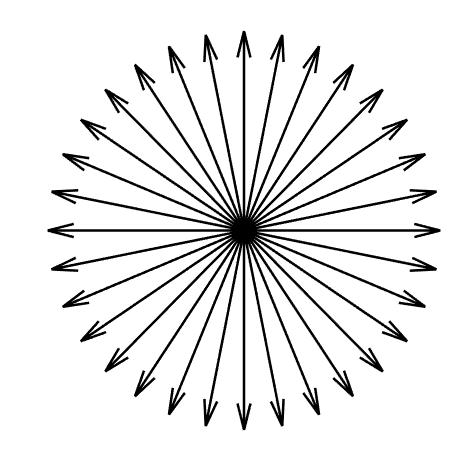
\includegraphics[width=0.4\textwidth]{../figure/arrow.png}}
        \subfigure[加权后$\mathbf{k}_0$]{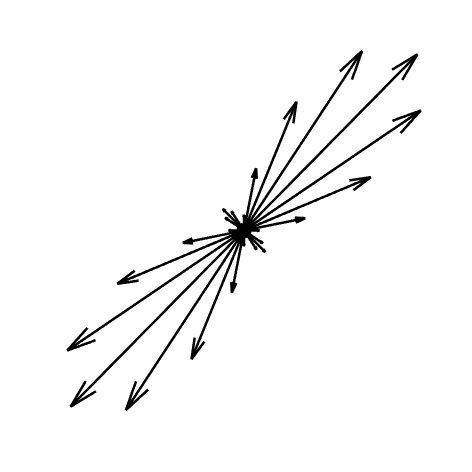
\includegraphics[width=0.4\textwidth]{../figure/processed_arrow.png}}
    \end{figure}
\end{frame}
\begin{frame}
    \frametitle{Husimi矢量}
    \centering
    \begin{tikzpicture}
        \draw[->] (-5.5,0) -- (5.5,0)node[right]{$x$};
        \draw[->] (0,-1.5) -- (0,4.5)node[right]{$y$};
        \draw[domain=1:4.5, red, thick]
            plot(\x,{4*2.71828^(-(\x-1)^2)});
        \draw[domain=-4.5:1, red, thick]
            plot(\x,{4*2.71828^(-(\x-1)^2)});
        \draw[domain=-5:0, blue, thick]
            plot(\x,{cos((\x*100)});
        \draw[domain=0:5, blue, thick]
            plot(\x,{cos((\x*100)});
        \node[above right, rounded corners] at (3,4) {红色:$\braket{\mathbf{r}|\mathbf{r}_0,\mathbf{k}_0,\sigma}$};
        \node[above right, rounded corners] at (3,3) {蓝色:$\braket{\mathbf{r}|\psi}$};
    \end{tikzpicture}
\end{frame}
%----------------------MMA---------------------------------%
\subsection{多模态分析算法}
\begin{frame}
    \frametitle{多模态分析算法}
    D. J. Mason在文中关于Multi-Modal Analysis (MMA)算法的描述如下所示
    \begin{figure}
        \centering
        \includegraphics[width=0.5\textwidth]{../MMA/MMA.png}
    \end{figure}
\end{frame}
\begin{frame}
    \frametitle{多模态分析算法}
    \begin{algorithm}[H] 
        \caption{多模态分析法(MAA:Multi-Modal Analysis)}
        \label{alg:maa}
        \begin{algorithmic}[1]
            \STATE 用M个波矢\{$\mathbf{k}^{test}_{i}$\}生成测试平面波$\psi=\mathrm{e}^{\mathrm{i}\mathbf{k}_i^{test}\cdot\mathbf{r}}$ ,将每个测试平面波用N个测试波矢\{$\mathbf{k}_j$\}(非测试平面波的波矢)生成模板集合的成员。
               两组波矢\{$\mathbf{k}_{i}^{test}\}$和$\{\mathbf{k}_{j}\}$都位于色散等值线上。每个模板(个数为M)存储的值为$\mathbf{u}_i$,$\mathbf{u}_i$的每一个成员对应于Husimi函数(式\ref{husimi:function})值;
            \label{alg:maastep:create}
            \STATE 相似程度的衡量标准由$\mathbf{d}_i=\mathbf{v}\cdot\mathbf{u}_i$给出,其中矢量$\mathbf{v}$表示Husimi矢量,$\mathbf{u}_i$表示在步骤\ref{alg:maastep:create})中的每个模板;
            \STATE 找出集合\{$d_i$\}的极大值和对应的波矢$\mathbf{k}^{test}_i$,并将它们保存下来;
            \STATE 带波矢$\mathbf{k}^{test}_{i}$的轨迹的贡献由重新加权的矢量决定$\mathbf{u}_{i}\frac{d_{i}}{\mathbf{u}_{i}\cdot\mathbf{u}_{i}}$;
            \STATE Husimi矢量减去加权后的模板矢量,即$\mathbf{v}_{i}\rightarrow\mathbf{v}_{i}-\mathbf{u}_{i}\frac{d_{i}}{\mathbf{u}_{i}\cdot\mathbf{u}_{i}}$
            \STATE 将$\mathbf{v}$的所有负元素设为零;
            \label {alg:maastep:loopend}
            \STATE 重复步骤\ref{alg:maastep:create})\,-\,\ref{alg:maastep:loopend})直到$\mathbf{d}_{i}$低于一个阈值;
            \STATE 矢量集合\{$d_{i}\,\mathbf{k}^{test}_i$\}近似为处理后的Husimi流;
        \end{algorithmic}
    \end{algorithm}
\end{frame}
\begin{frame}[allowframebreaks]
    \frametitle{MMA的思想}
    将测试平面波与未知波的Husimi函数值进行比较,找到相似之处。
    \begin{figure}
        \centering
        \subfigure[$\psi^{test}=\mathrm{e}^{\mathrm{i}\mathbf{k}_{i}^{test}\cdot\mathbf{r}}$]
        {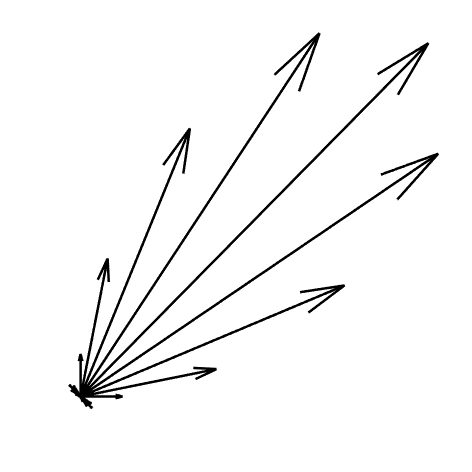
\includegraphics[width=0.42\textwidth]{../figure/PsiTest.png}}
        \qquad
        \subfigure[$\psi=\alpha\cos{(\mathrm{i}\mathbf{k}_1\cdot\mathbf{r})}+\beta\cos{(\mathrm{i}\mathbf{k}_2\cdot\mathbf{r})}$]
        {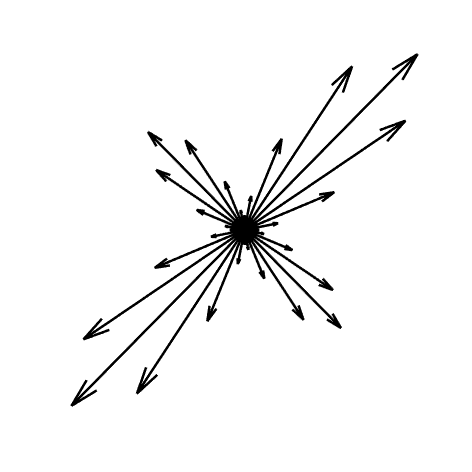
\includegraphics[width=0.42\textwidth]{../figure/PsiC.png}}
    \end{figure}
    \begin{columns}
        \begin{column}{0.62\textwidth}
            \begin{center}
                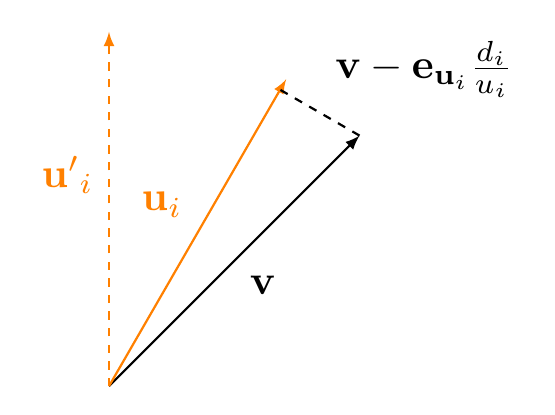
\begin{tikzpicture}[thick]
                    \coordinate (O) at (0,0);
                    \draw[-latex] (O) --node[below right, scale=1.5] {$\mathbf{v}$} (45:4.5);
                    \draw[-latex, orange] (O) --node[above left, scale=1.5] {$\mathbf{u}_i$} (60:4.5);
                    
                    \draw[dashed] (45:4.5) --node[above right, scale=1.5] {$\mathbf{v}-\mathbf{e}_{\mathbf{u}_{i}}\frac{d_i}{u_i}$} (60:4.3466);
                    \draw[-latex, orange, dashed] (O) --node[above left, scale=1.5] {$\mathbf{u'}_i$} (90:4.5);
                    %垂线%
                \end{tikzpicture}
            \end{center}
        \end{column}
        \begin{column}{0.3\textwidth}
            {\normalsize 寻找$d_i$最大值}
            \Large
            \begin{equation*}
                d_i = \mathbf{v}\cdot\mathbf{u}_i
            \end{equation*}
            {\normalsize 其中$|\mathbf{v}| = 1,|\mathbf{u}_i| = 1$}
        \end{column}
    \end{columns}
\end{frame}
\begin{frame}[allowframebreaks]
    \frametitle{\textbf{MMA}的看法}
    \begin{enumerate}
%
    \item 原文:A set of \textcolor{blue!90}{templates} on N wave vectors \{$\mathbf{k_j}$\} is 
                    created for the wave functions $\psi=\mathrm{e}^{\mathrm{i}\mathbf{k}_{i}^{test}\cdot\mathbf{r}}$ 
                    generated by the M wave vectors $\{\mathbf{k}_{i}^{test}\}$. Both sets of wave vectors lie along the 
                    dispersion contour. Each \textcolor{blue!90}{template} is stored as a vector of values $u_i$ (length M) 
                    and corresponds to eq. (12) along $k_j$.\\
          理解:
        \begin{itemize}
        \item 第一句话的含义应该是用M个$\{\mathbf{k}_{i}^{test}\}$产生一个模板(templates)集\{$k_{i}^{test}$\},从最后一句话
            可以推断每个模板$\mathbf{u}_i$应该是个由\{$k_j$\}组成的向量集。
        \item 最后一句说$\mathbf{u}_i$的每个值对应于(\ref{husimi:function})式(Husimi函数)同时在$k_j$方向上。因此,我推断$\mathbf{u}_i = [ \mathbf{u}_i^{1}\ \mathbf{u}_i^{2}\ \cdots\ \mathbf{u}_i^{N}]$,
            其中$\mathbf{u}_i^{j}=\mathrm{Hu}(\psi=\mathrm{e}^{\mathrm{i}\mathbf{k}_{i}^{test}\cdot\mathbf{r}},k_j)$
        \item 对于第二句中提到的色散等值线,个人觉得应该是说$\mathbf{k}_{i}^{test}=\frac{\sqrt{2mE^{test}}}{\hbar}$和
                $\mathbf{k}_{j}=\frac{\sqrt{2m[E-V(\mathbf{r})]}}{\hbar}$中的$E$和$E^{test}$位于同一条等值线上,即$E=E^{test}$
        \end{itemize}
%
    \item 原文:The metric given by $d_i=\mathbf{v}\cdot\mathbf{u}_i$, where the vector $\mathbf{v}$ represents the \textcolor{red!80}{Husimi vector}, is computed for
                        each \textcolor{blue!90}{template} in step 1).\\
          理解:
            \begin{itemize}
                \item Husimi矢量应该不是一个简单的矢量,而是一个矢量集\{$\mathbf{v}^{j}$\},即$\mathbf{v}=[\mathbf{v}^1\ \mathbf{v}^2\ \cdots\ \mathbf{v}^N]$
                \item 因此,我认为$d_i$应该不是一个标量而是一个$N\times N$张量,即$d_i^{j,j'}=\mathbf{v}^{j}\cdot\mathbf{u}_{i}^{j'}$\colorbox{red!60}{这点与原文中不同}
                \item 我觉得这一步是为测出$\psi_c$的波矢$\mathbf{k}$与测试平面波的波矢$\mathbf{k}_i^{test}$的相近程度。
            \end{itemize}
%
    \item 原文:The maximum of the set \{$d_i$\} and the corresponding wave vector $\mathbf{k}_{i}^{test}$ are stored.\\
          理解:
            \begin{itemize}
                \item 这一步应该是找出与$\psi_c$的波矢$\mathbf{k}$相近的测试平面波的波矢$\mathbf{k}_i^{test}$。
                \item 我个人认为应该将\{$d_i$\}集合中的所有列放在一起比较,可以加快收敛速度。(还没尝试)
                    \begin{equation*}
                        d_i=  
                        \begin{bmatrix}
                            \mathbf{v}^{1}\cdot\mathbf{u}_i^{1}&\cdots&\mathbf{v}^{1}\cdot\mathbf{u}_i^{N}\\
                            \vdots & \ddots &\vdots\\
                            \mathbf{v}^{N}\cdot\mathbf{u}_i^{1}&\cdots&\mathbf{v}^{N}\cdot\mathbf{u}_i^{N}\\
                        \end{bmatrix}
                    \end{equation*}
                \item 我的操作是找出$\mathbf{d}_i$中元素的最大值的行${j_max}$与列${j'_max}$
            \end{itemize}
    \item 原文:The contribution of the trajectory with wave vector $\mathbf{k}_{i}^{test}$ is determined by 
                        the vector $\mathbf{u}_i\frac{d_i}{\mathbf{u}_i\cdot\mathbf{u}_i}$\\
          理解:
            \begin{itemize}
                \item 从这句话说重新加权的矢量$\mathbf{u}_i\frac{d_i}{\mathbf{u}_i\cdot\mathbf{u}_i}$由$\mathbf{k}_{i}^{test}$
                        决定。因为,$d_{i}^{j,j'}$的大小由$\mathbf{u}_{i}^{j'}$决定,而$\mathbf{u}_{i}^{j'}$又由$\mathbf{k}_{i}^{test}$决定。
                \item 测试的平面波的$\mathbf{k}_i^{test}$越接近$\psi_c$的$\mathbf{k}$,$d_i$的值越大。
            \end{itemize}
%
    \item 原文:The re-weighted template vector is subtracted from the \textcolor{red!80}{Husimi vector}, i.e.$\mathbf{v}_i \rightarrow \mathbf{v}_i - \mathbf{u}_i\frac{d_i}{\mathbf{u}_i\cdot\mathbf{u}_i}$\\
          理解:
            \begin{itemize}
                \item 当找出与$\mathbf{u}_{i}^{j'}$相匹配的$\mathbf{v}^{j}$后,应减去它们之间相同的部分,防止在下次迭代计算中误判。
                \item 计算操作可表达为$\mathbf{v'}^{j_{max}}=\mathbf{v}^{j_{max}}-\mathbf{u}_{i}^{j'_{max}}\frac{d_{i}^{j_{max},j'_{max}}}{\mathbf{u}_{i}^{j'_{max}}\cdot\mathbf{u}_{i}^{j'_{max}}}$
            \end{itemize}
    \item 原文:All negative elements of $\mathbf{v}$ are set to zero.\\
          理解:
            \begin{itemize}
                \item 我觉得这一步是为加快收敛速度,已判断出的$v^{j'_{max}}$不再被误判。
                \item 可能这句话另有含义,但在我想出的这套算法中没有体现。
            \end{itemize}
    \item 原文:Steps 1)–6) are repeated until the metric $d_i$ dips
            below a threshold.\\
          理解:
            \begin{itemize}
                \item 循坏停止的条件$\max{d_i}<eps$,
                \item 从这点说明$d_i\mathbf{k}_{i}^{test}$的方向应该是流的方向。
            \end{itemize}
    \end{enumerate}
\end{frame}
%-------------------------------------------------------------%
%
%-------------------------------------------------------------%
\section{复现的结果}
\subsection{未处理的Husimi图}

\begin{frame}
    \frametitle{文中的图2}
    \begin{figure}
        \centering
        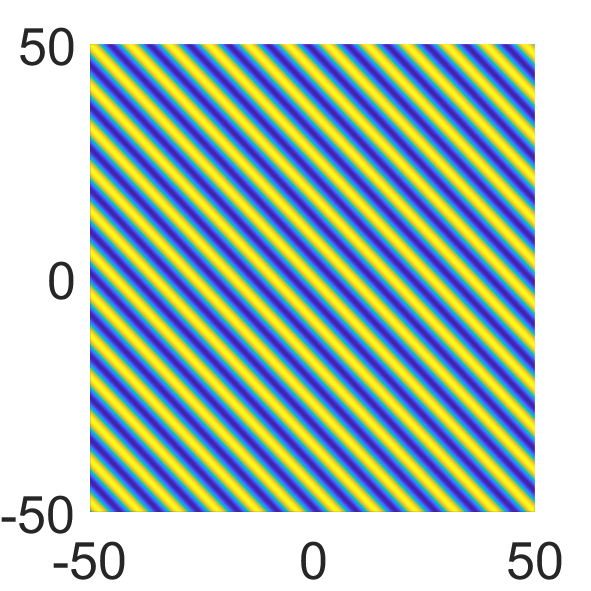
\includegraphics[width = 0.2\textwidth]{../figure/PsiA2.png}
        \quad
        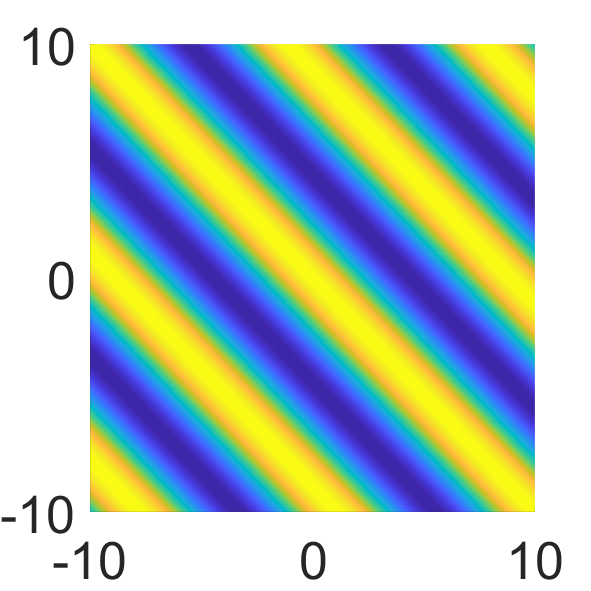
\includegraphics[width = 0.2\textwidth]{../figure/PsiA10.png}
        \quad
        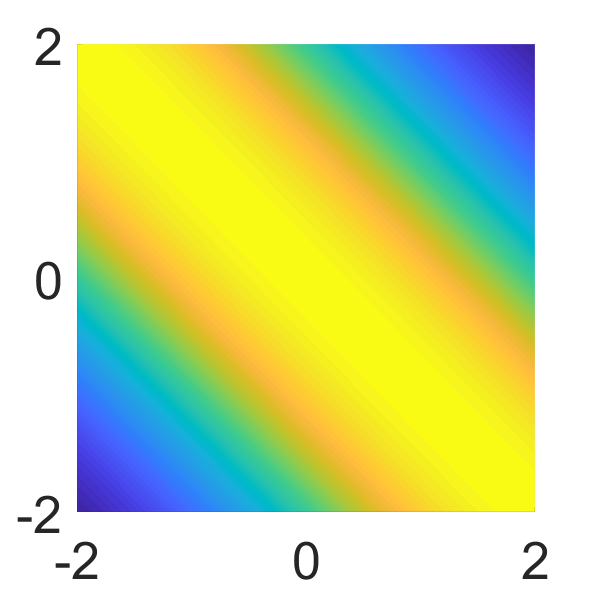
\includegraphics[width = 0.2\textwidth]{../figure/PsiA50.png}
        \quad
        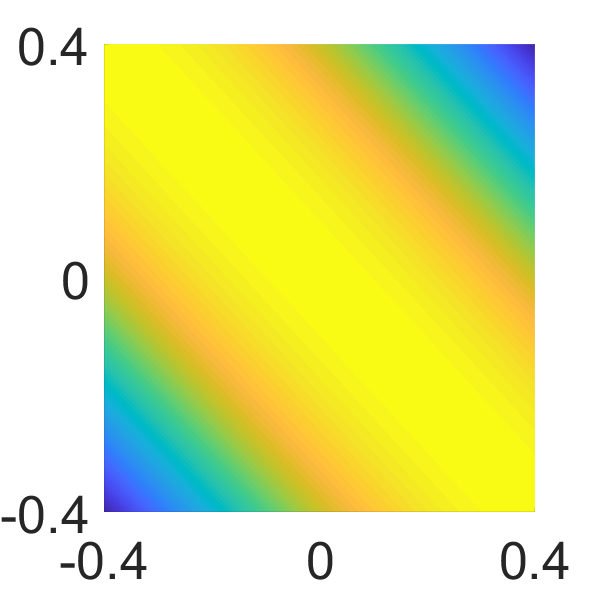
\includegraphics[width = 0.2\textwidth]{../figure/PsiA250.png}
        \subfigure[$ 2\% $]{
            \centering        
            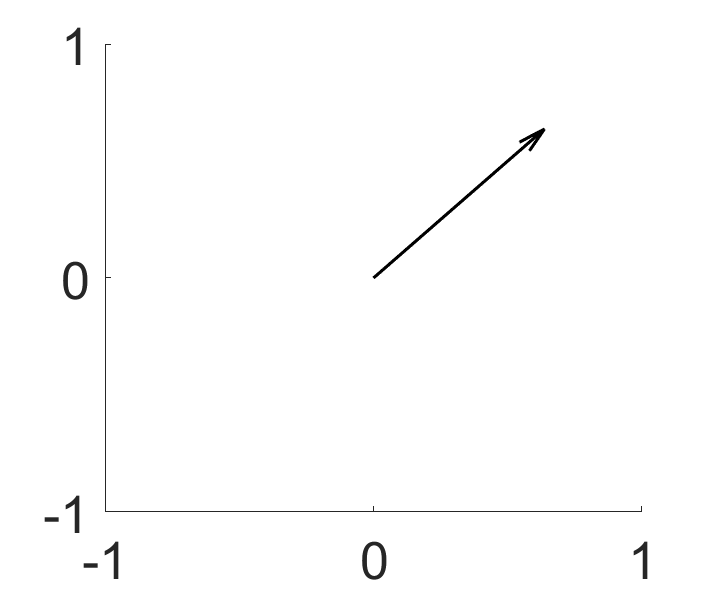
\includegraphics[width = 0.2\textwidth]{../figure/HuA2.png}
        }
        \subfigure[$ 10\% $]{
            \centering
            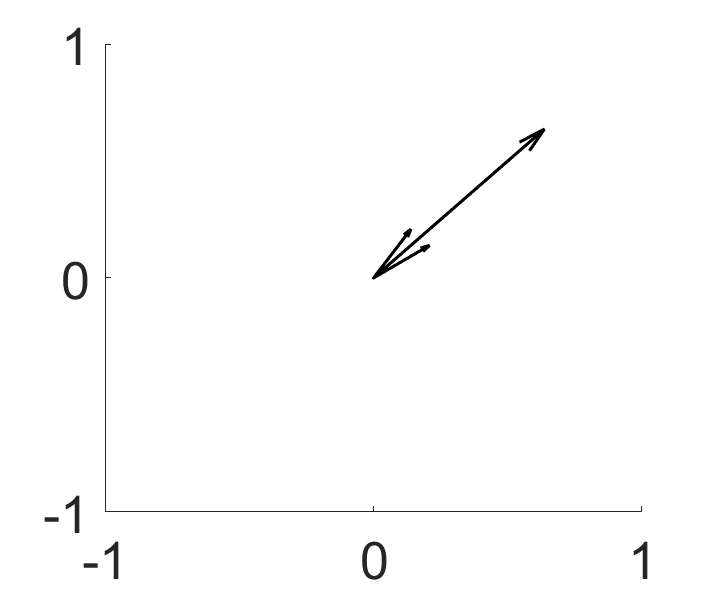
\includegraphics[width = 0.2\textwidth]{../figure/HuA10.png}
        }
        \subfigure[$ 50\% $]{
            \centering
            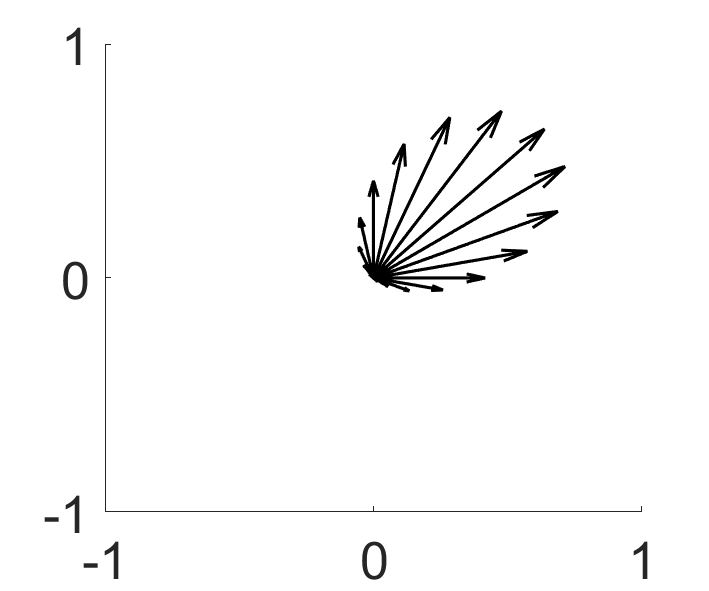
\includegraphics[width = 0.2\textwidth]{../figure/HuA50.png}
        }
        \subfigure[$ 250\% $]{
            \centering
            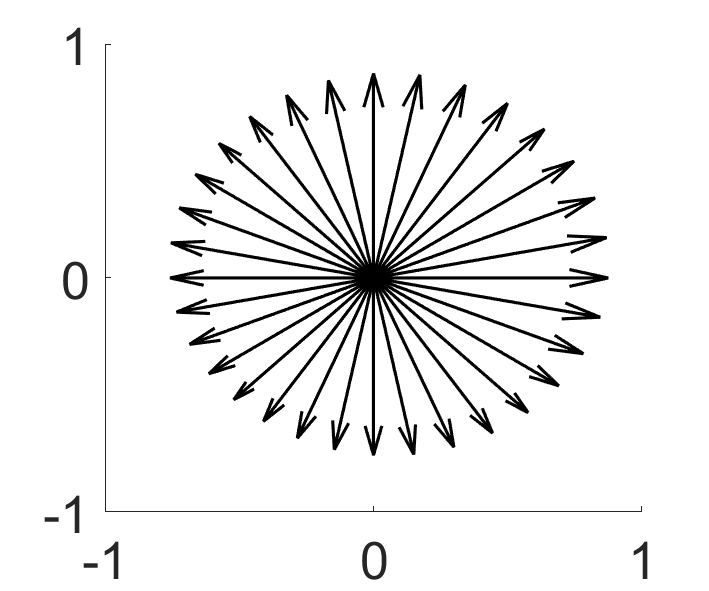
\includegraphics[width = 0.2\textwidth]{../figure/HuA250.png}
        }
       \caption{$\psi_A(\mathbf{r})=\mathrm{e}^{\mathrm{i}\mathbf{k}\cdot\mathbf{r}}$,小图$\Delta k/k$}         
    \end{figure}
\end{frame}
\begin{frame}
    \frametitle{文中的图2}
    \begin{figure}
        \centering
        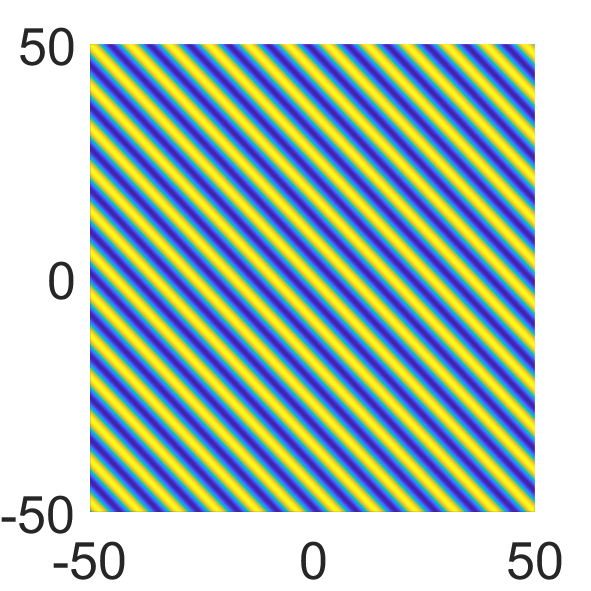
\includegraphics[width = 0.2\textwidth]{../figure/PsiB2.png}
        \quad
        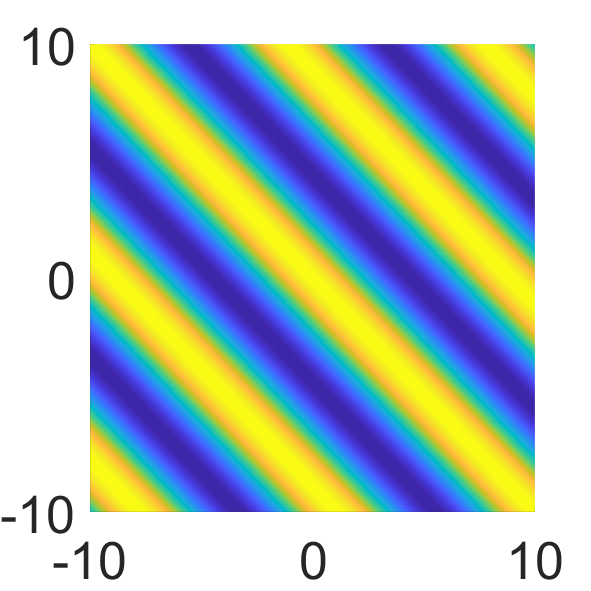
\includegraphics[width = 0.2\textwidth]{../figure/PsiB10.png}
        \quad
        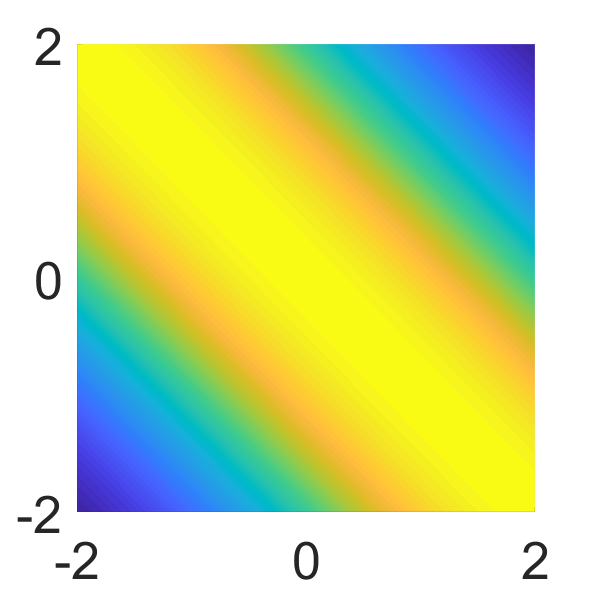
\includegraphics[width = 0.2\textwidth]{../figure/PsiB50.png}
        \quad
        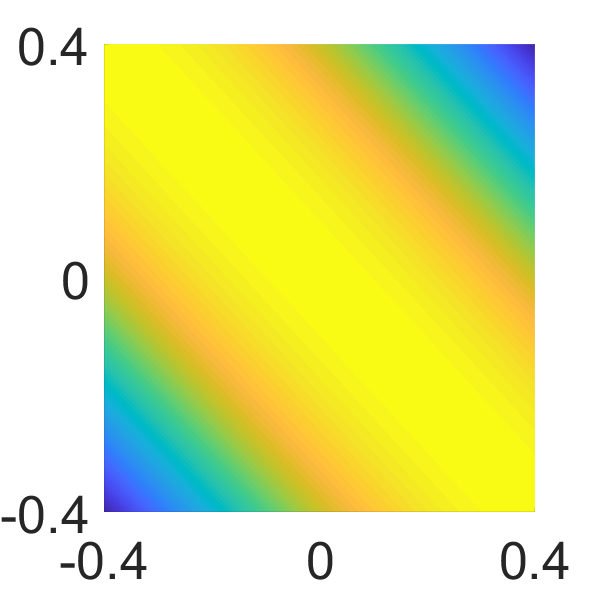
\includegraphics[width = 0.2\textwidth]{../figure/PsiB250.png}
        \subfigure[$ 2\% $]{
            \centering        
            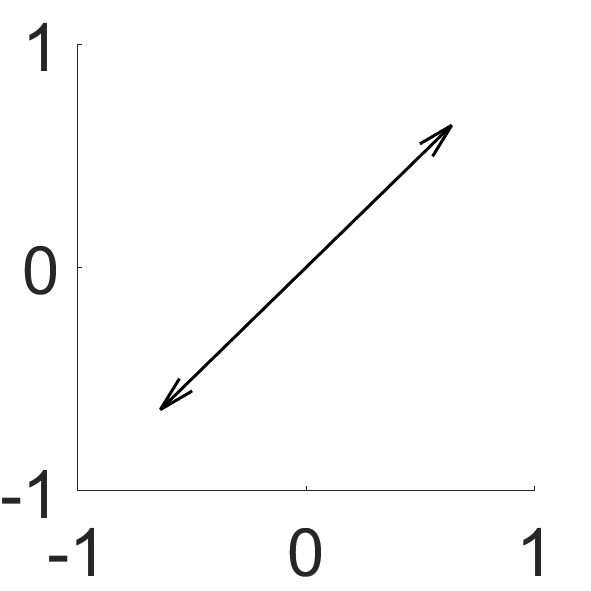
\includegraphics[width = 0.2\textwidth]{../figure/HuB2.png}
        }
        \subfigure[$ 10\% $]{
            \centering
            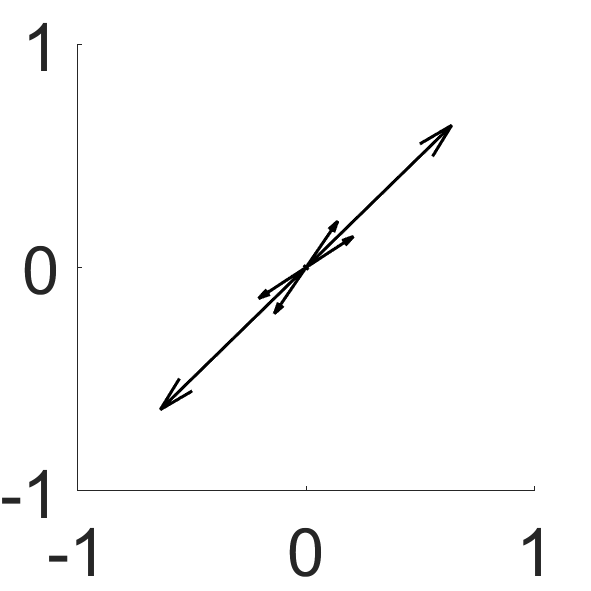
\includegraphics[width = 0.2\textwidth]{../figure/HuB10.png}
        }
        \subfigure[$ 50\% $]{
            \centering
            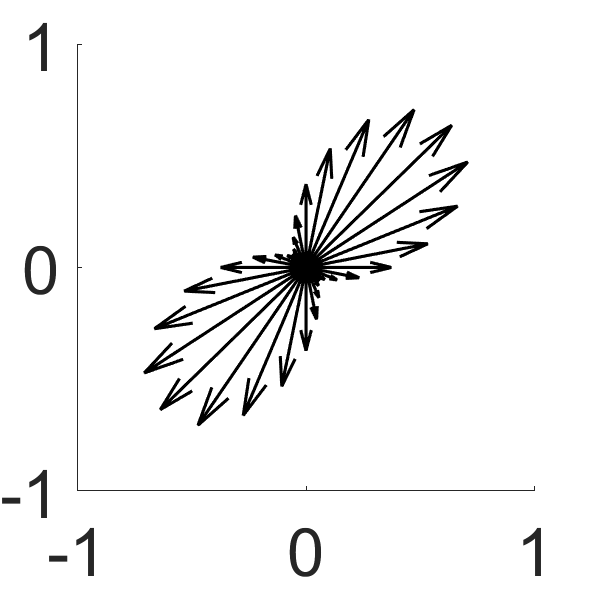
\includegraphics[width = 0.2\textwidth]{../figure/HuB50.png}
        }
        \subfigure[$ 250\% $]{
            \centering
            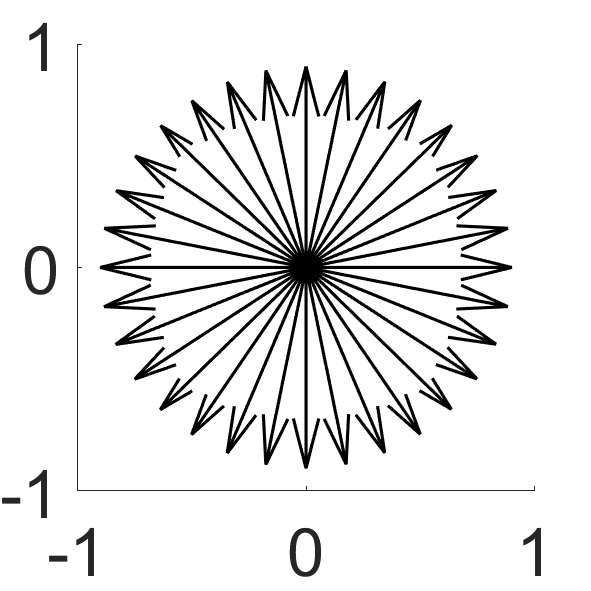
\includegraphics[width = 0.2\textwidth]{../figure/HuB250.png}
        }
       \caption{$\psi_B(\mathbf{r})=\cos (\mathbf{k}\cdot\mathbf{r}$,小图$\Delta k/k$}         
    \end{figure}
\end{frame}
\begin{frame}
    \frametitle{文中的图3}
    \begin{figure}[h]
        \centering
        \subfigure[$ \Delta k /k = 30\%$ 时的Husimi图]
        {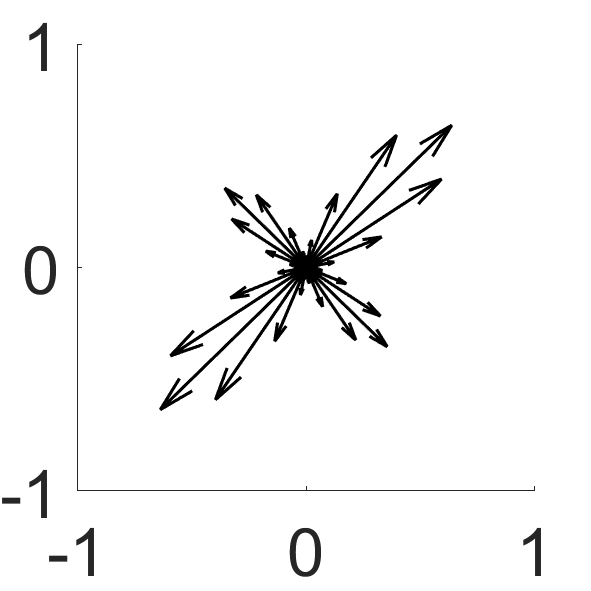
\includegraphics[width = 0.42\textwidth]{../figure/HuC30.png}}
        \qquad
        \subfigure[$ \Psi_C = \alpha\cos ({\mathrm{i}\mathbf{k}\cdot\mathbf{r}}) + \beta\cos ({\mathrm{i}\mathbf{k}\cdot\mathbf{r}})$]
        {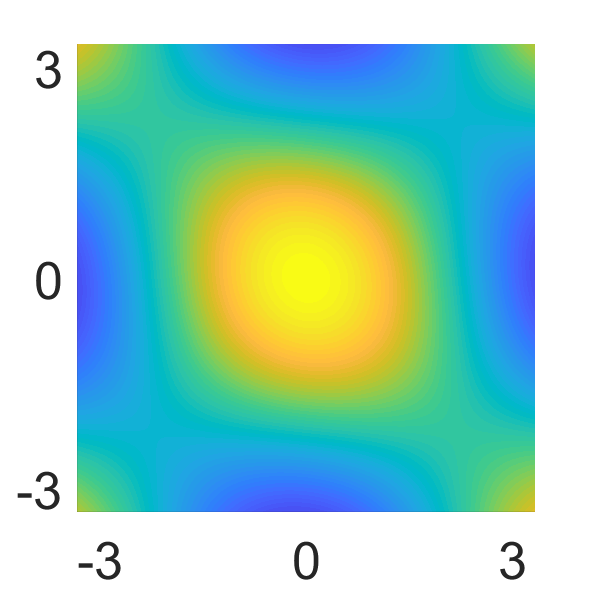
\includegraphics[width = 0.42\textwidth]{../figure/PsiC30.png}}
        \caption{Husimi图}
    \end{figure}
\end{frame}
%
%--------------------------------------------------------------%
\subsection{处理过的Husimi图}
\begin{frame}
    \frametitle{利用MMA算法处理过的$\psi_c$}
    \begin{figure}
        \centering
        \subfigure[]{
            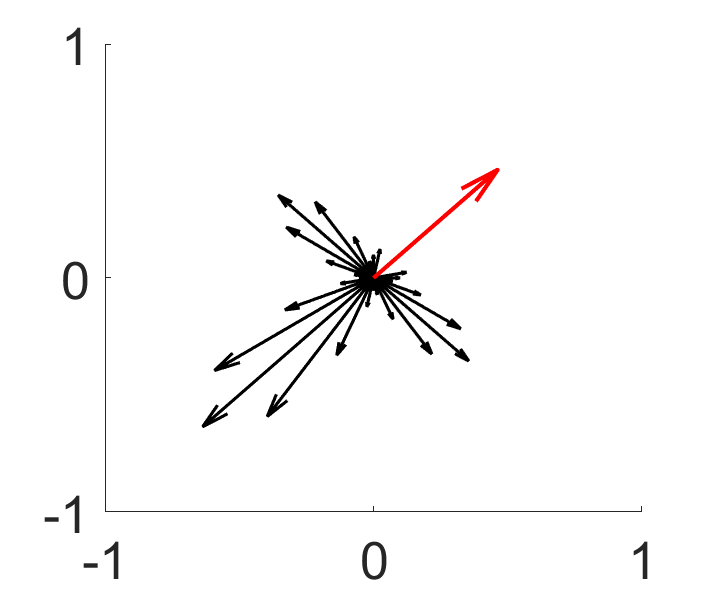
\includegraphics[width = 0.28\textwidth]{../figure/HuC1.png}
        }
        \subfigure[]{
            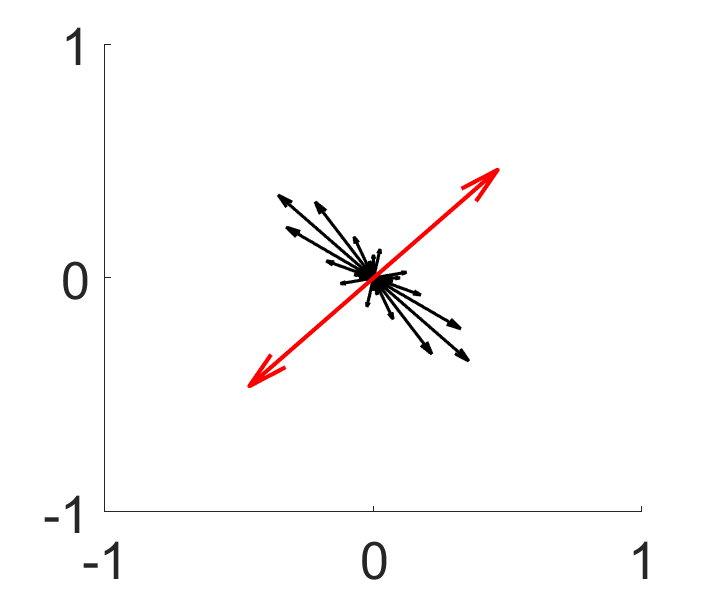
\includegraphics[width = 0.28\textwidth]{../figure/HuC2.png}
        }\\
        \subfigure[]{
            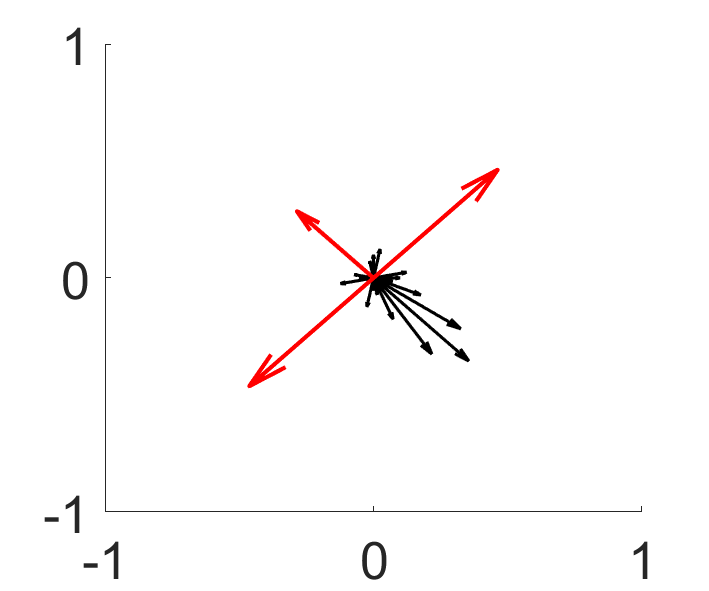
\includegraphics[width = 0.28\textwidth]{../figure/HuC3.png}
        }
        \subfigure[]{
            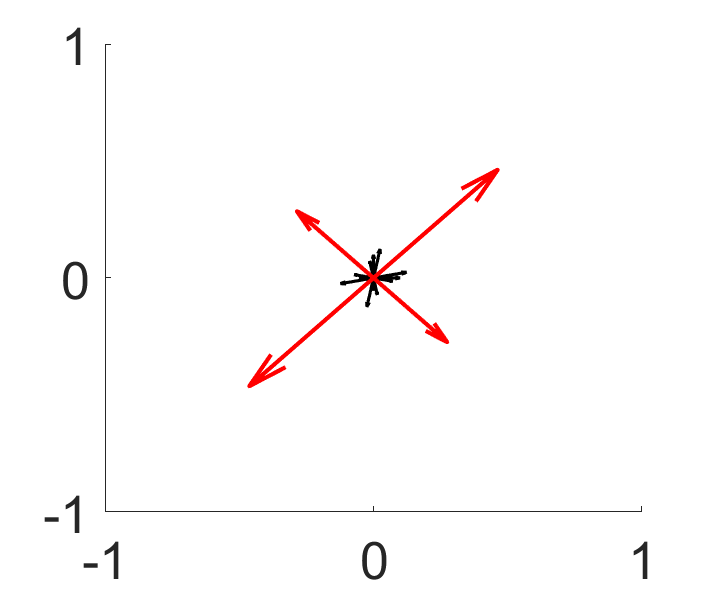
\includegraphics[width = 0.28\textwidth]{../figure/HuC4.png}
        }
    \end{figure}
\end{frame}
\end{document}